% !TeX root = RJwrapper.tex
\title{USstocks}
\author{by Duncan Cummings, David Kane and Andy Yu Zhu Yao}

\maketitle

\abstract{ \\

The \pkg{USstocks} package compiles daily stocks observation of 3081 top performing US companies from 1997-2008, with indictors such as daily returns, trading price, volume, and market capitalization. The data originated from Kane Capital Management's quantitative strategies department. The \pkg{USstocks} package cleaned the original data, and merged all valuable information into a single data frame that is user-friendly and easy to work with. In this vignette, we demonstrate some simple techniques and strategies one could employ to explore this rich data set. Specifically, we explore the performance of stocks across time, the market share of different industries, difference in stock volatility across sectors/industries, and the companies that were part of the Dot-com bubble phenomena.
}

\section{Background} 

The original data for \pkg{USstocks} comes from the \pkg{ws.data} package gathered by Kane Capital Management, a hedge fund in operation from 2004 to 2010. The fund maintained a research database of daily equity data for their quantitative strategies, which was determined by a methodical selection process performed at the end of every year. Starting on December 31, 1998, Kane Capital observed all the U.S. stocks over the past year and selected the top 1,500 performing stocks measured by market capitalization. For the following 9 years (1998 - 2007) the process was repeated at the end of each year, culminating in the \pkg{ws.data} package of daily stock information for 3,083 companies that were on the top 1500 list for atleast one year. \\

In \pkg{USstocks}, we improved the \pkg{ws.data} datasets in two ways. First, we merged all the information into one single data.frame. In the original package, there were multiple data.frames each containing separate information about stocks, such as daily information, yearly information, and sector/industry information. The merged dataframe is called \code{stocks} in our \pkg{USstocks} package, and could be loaded by the simple command \code{data(stocks)}. \\

Second, in our examination of the original dataset from Kane Capital, we found certain questionable outliers and cleaned those up. For all intents and purposes of this package, we decided that it was best for the user to perform stock analysis without having to worry about these questionable outliers. 

\section{Cleaning Up the Original Stocks Dataset}

Specifically, certain questionable outliers in \pkg{ws.data} were removed. In the original data set, Kane Capital's methodology was that once a company was recorded as top 1500 for one year, the company's information in the subsequent years would be collected regardless of performance. This led to some suspicious observations as certain companies still had stock information (with unreasonable figures, of course) after the company declared bankruptcy. After cross-verifying with historical data, we found that most of these companies were part of the DotCom bubble. Thus, we removed these statistically insignificant observations from our dataset. A detailed audit trail of the steps we've taken to remove these suspicious observations could be found on our GitHub. Here, we simply summarize the list of stocks that were removed: \\

\begin{tabular}{ | p{4cm} | p{4cm} | p{4cm} |}
    \hline
    Name of Company & Observations Removed & Reason for Removal \\ \hline
    CHATHAM CORP-DE & every observation & unreasonably low volume, high return \\ \hline
    STRATOSPHERE CORP & every observation & meaningless observation (company filed for bankruptcy)  \\ \hline
    CYCLELOGIC INC & 2 outlying observations removed & inconsistent with data trend, unreasonably high returns \\ \hline
    METRICOM INC & 1 outlying observations removed & inconsistent with data trend, unreasonably high returns \\ \hline
    MARCHFIRST INC & every observation after 2002 & DotCom bubble, meaningless observation after bankruptcy \\ \hline
    RHYTHMS NETCONNECTIONS INC & every observation after 2002 & DotCom bubble, meaningless observation after bankruptcy \\ \hline
    CLARENT CORP & every observation after 2002 & DotCom bubble, meaningless observation after bankruptcy \\ \hline
    LUMINANT WORLDWIDE CORP & 1 outlying observations removed & inconsistent with data trend, unreasonably high returns \\ \hline
    ACCRUE SOFTWARE INC & every observation & security fraud, insignificant observation \\ \hline
    WEBVAN GROUP INC & every observation after 2001 & DotCom bubble, meaningless observation after bankruptcy \\ \hline
    SCIENT INC & every observation after 2002 & DotCom bubble, meaningless observation after bankruptcy \\ \hline
    ENGAGE INC & every observation after 2003 & DotCom bubble, meaningless observation after bankruptcy \\ 
    \hline
\end{tabular}
\newline

\section{Getting Started}

\begin{example}
  install_github("yuzhuyao/USstocks")
  library(USstocks)
  data(stocks)
\end{example}

\section{The USstocks Data}

\begin{tabular}{|r|l|}
  \hline
  \multicolumn{2}{|c|}{Variables and Meaning} \\
  \hline
  \dfn{id} & unique security identifier (randomly generated?) \\
  \dfn{symbol} & stock exchange ticker \\ 
  \dfn{v.date} & date of observation \\ 
  \dfn{price.unadj} & unadjusted price \\ 
  \dfn{price} & price (adjusted) \\ 
  \dfn{volume.unadj} & unadjusted volume \\ 
  \dfn{volume} & volume (adjusted) \\ 
  \dfn{tret} & total returns (how is it defined?) \\ 
  \dfn{m.sec} & sector to which the stock belongs \\ 
  \dfn{m.ind} & industry to which the stock belongs \\
  \dfn{name} & company name \\
  \dfn{year} & year \\
  \dfn{cap.usd} & market capitalization (of the year) \\ 
  \dfn{top.1500} & boolean indicating whether the stock is part of the top 1500 performing in that year \\
  \hline
\end{tabular}

\newpage

\section{Exploring the Data}

Before we get started, note that there are two packages that are extremely helpful for working with our \code{stocks} data.frame. The package \pkg{dplyr} enables us to perform basic SQL operations on our data.frame extremely efficiently, and \pkg{ggplot2} helps with data trend visualization. Import them by calling: \code{library(dplyr)} and \code{library(ggplot2)}. Now, let's get started with looking at IBM's stock from 1998 to 2007. \\

\noindent Let's get started with what the data frame looks like for a specific stock (e.g. IBM) (FIX THE VISUALIZATION):

\begin{example}
> stocks %>%
+  filter(symbol == "IBM") %>%
+  arrange(v.date) %>% head
\end{example}

\begin{figure}[h!]
  \centering
    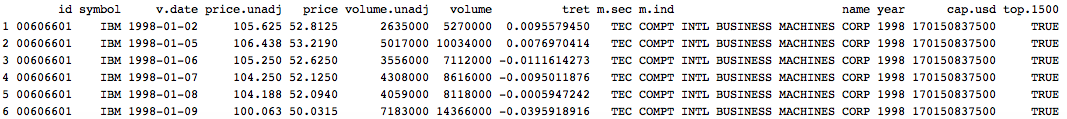
\includegraphics[width=1.2\textwidth]{IBM1}
\end{figure}

\noindent We can also visualize the price of the IBM stock over the years (\textbf{Figure 1}):

\begin{example}
> stocks %>%
+  filter(symbol == "IBM") %>%
+  arrange(v.date) %>%
+  ggplot() + geom_point(aes(x = v.date, y = price))
\end{example}

\begin{figure}[h!]
  \centering
    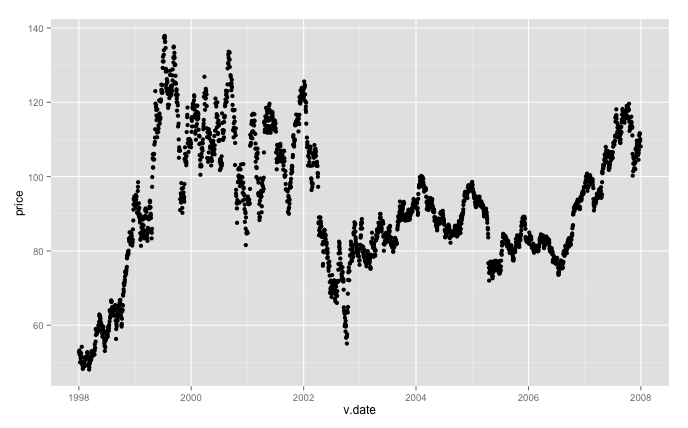
\includegraphics[width=0.8\textwidth]{IBM2}
  \caption{Price of IBM's stock from 1998 to 2007}
\end{figure}

\noindent We could also take a look at some of the key statistics for, say Microsoft: 

\begin{example}
> stocks %>%  
+  filter(symbol == "MSFT") %>%
+  summarise_each(funs(mean, median), volume, volume.unadj, price, price.unadj)
\end{example}

\noindent We could also take a look at market share across sectors

\begin{example}
> x %>% select(name, m.sec, year, cap.usd) %>% unique %>% filter(year == 1998) -> y
> y %>% filter (!is.na(cap.usd)) %>% group_by(m.sec) 
+   %>% summarise(sector_total_1998 = sum(cap.usd)) -> y 
> y %>% ggplot(aes(x = "", y = sector_total_1998, fill = m.sec), label = m.sec) + 
+   geom_bar(width = 1, stat = "identity") + coord_polar(theta="y") 
\end{example}

\begin{figure}[h!]
  \centering
    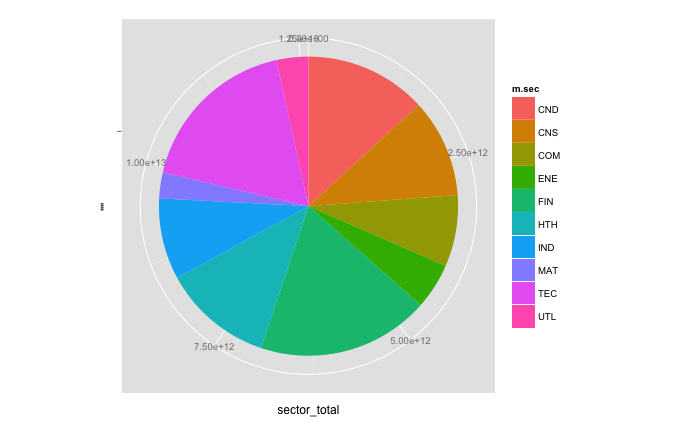
\includegraphics[width=0.9\textwidth]{PIE1}
  \caption{Market share of different sectors for the top 1500 companies in 1998}
\end{figure}

\section{Cross Sector/Industry Volatility Comparison}

\noindent We could look at the largest positive and negative daily return across different sectors. As we could see below, the Technology sector contains both the largest and negative daily returns, whereas the Energy sector is much more stable(\textbf{Figure 3, 4}). 

\begin{example}
> stocks  %>% 
+  group_by(v.date, m.sec)  %>% 
+  filter(row_number(desc(tret)) == 1)  %>% 
+  ggplot(aes(x = v.date, y = tret)) + geom_point() + facet_wrap(~m.sec)

+ stocks  %>% 
+  group_by(v.date, m.sec)  %>% 
+  filter(row_number(desc(tret)) == n())  %>% 
+  ggplot(aes(x = v.date, y = tret)) + geom_point() + facet_wrap(~m.sec)
\end{example}

\begin{figure}[ht]
\centering
\begin{minipage}[b]{0.45\linewidth}
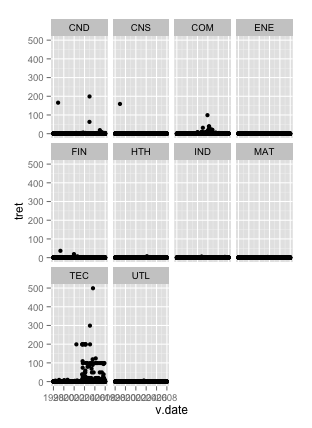
\includegraphics[width=.8\linewidth]{DEMO1}
\caption{largest positive returns across sectors}
\end{minipage}
\quad
\begin{minipage}[b]{0.45\linewidth}
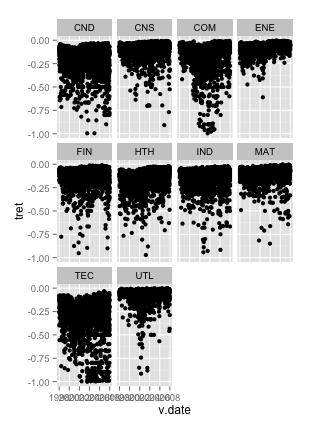
\includegraphics[width=.8\linewidth]{DEMO2}
\caption{largest negative returns across sectors}
\end{minipage}
\end{figure}

First, let's take a glance into the different standard deviation in returns across different sectors(\textbf{Figure 5}): 

\begin{example}
> x  %>% 
+   group_by(v.date, m.sec)  %>% 
+   mutate(sd_ret = sd(tret, na.rm = TRUE)) %>%
+   distinct(v.date, m.sec) %>%
+   ggplot(aes(x = v.date, y = sd_ret)) + geom_point() + facet_wrap(~m.sec)
\end{example}
\begin{figure}[h!]
  \centering
    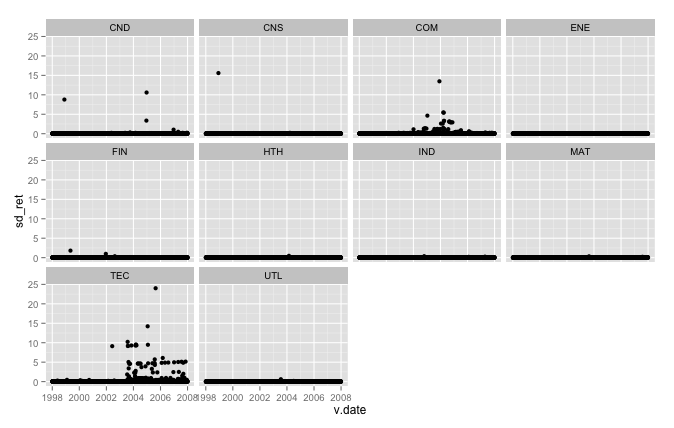
\includegraphics[width=0.8\textwidth]{VOL1}
  \caption{Standard Deviation in returns across sectors}
\end{figure}

\noindent From the plots above, it seems like certain sectors (e.g. Technology) are much more volatile than others. But how can we look into that phenomenon and understand more about what is going on? 

\section{A Glimpse into the Dotcom Bubble!}

\noindent Webvan was a online delivery grocery business that declared bankruptcy in 2001. It was named the largest dot-com flop in history by CNET in 2008. Wouldn't it be interesting to take a look at Webvan's stock across time?

\begin{example}
> x %>% filter(name == "WEBVAN GROUP INC", !is.na(price), year < 2002) %>% 
+   ggplot(aes(x=v.date, y = price)) + geom_point()
\end{example}
\begin{figure}[h!]
  \centering
    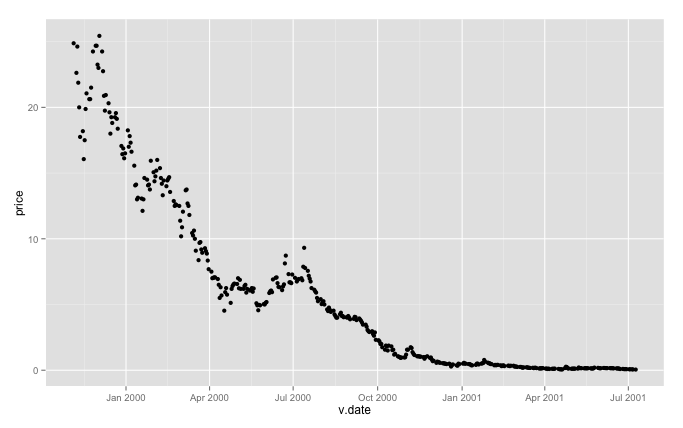
\includegraphics[width=0.8\textwidth]{WEBVAN}
  \caption{Webvan's Stock Price during the Dot-com bubble burst}
\end{figure}

\noindent As we could see from the figure above, as the Dot-com bubble bursted, the price of Webvan's stock dropped exponentially within a year, until it declared bankruptcy in July 2001.  

\section{Summary}

\bibliography{Kane}

\section{Authors}

\address{Duncan Cummings\\
  Williams College\\
  Williamstown, MA\\
  USA\\}
\email{dmc3@williams.edu}

\address{David Kane\\
  Hutchin Hill Capital\\
  Address\\
  Country\\}
\email{Dave.Kane@gmail.com}

\address{Andy Yu Zhu Yao\\
  Williams College\\
  Williamstown, MA\\
  USA\\}
\email{andy.yu.zhu.yao@williams.edu}
